\documentclass{report}

\usepackage[utf8]{inputenc}
\usepackage[francais]{babel}
\usepackage{graphicx}
\usepackage{setspace}
\renewcommand{\thesection}{\arabic{section}}
\begin{document}
\onehalfspacing
\title{%
    \begin{minipage}\linewidth
        \centering
        ISTY-IATIC-3
        \vskip 3pt
        \large Projet-Système - Dossier Momonga FS
    \author{Mathieu BRETTE \and Pablo BOURDELAS \and Sébastien POIROT\and Guillaume RYCKAERT}
    \end{minipage}
 }
 \maketitle

 \section*{Introduction}

 Le but de ce projet est de créer un Système de fichiers(SGF) en C, en implémentant des primitives, un shell, ainsi que la sauvegarde/recharge du disque.

Nous avons donc choisi de créer un SGF travaillant sur un disque virtuel, stocké sous la forme d'un fichier nommé vdisk. Le SGF devra être capable de créer un disque virtuel, de créer et supprimer des fichiers et des dossiers, ainsi que d'afficher leur contenu.
\vskip 10pt
\begin{figure}[ht!]
        \centering
        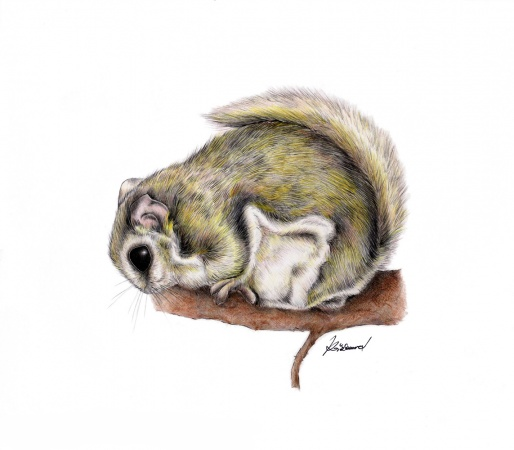
\includegraphics[width=125mm]{momonga.png}
\end{figure}

\newpage

\section*{Structure du disque}
Le disque est composé des différentes structures suivantes:
\begin{itemize}
\item Le SuperBlock
\item Les inodes
\item L'Inode Bitmap
\item La Block Bitmap
\item Les Data
\end{itemize}

\subsection*{Le SuperBlock}
Le SuperBlock contient les informations essentielles du disque,\\comme par exemple: 
\begin{itemize}
\item Le nombre total d'inodes sur le disque
\item Le nombre total de blocks de données sur le disque
\item Le nombre de blocks libres
\item Le nombre d'inodes libres
\item La taille des blocks (en bytes)
\item Ainsi que le numéro du premier block de données
\end{itemize}
Le superblock est chargé en même temps que le disque, dans le cas de la création d'un disque, il est automatiquement crée. Nous acons choisi de déclarer le SuperBlock en global, car il est utilisé dans de nombreuses fonction du SGF.
\subsection*{Les inodes}
Chaque inode représente un fichier/dossier sur le disque. L'inode fournit les informations suivantes:
\begin{itemize}
    \item La taille des données du fichier.\footnote{Pour les dossiers, voir plus bas.}
    \item Une valeur représentant les droits d'acces, ainsi que la nature(fichier/dossier).
    \item Un tableau de 15 numéros de blocks, les 12 premiers représentent les blocks contenant les données du dossier/fichier.Le 13ème est le numéro de block indirect: ce block contient des numéros de blocks appartenant au fichier.De même pour le 14ème block qui est double indirect, et pour le 15ème, qui est triple indirect.
    \item Un nombre représentant la dernière fois que le fichier a été modifié.\footnote{Non implémenté}
    \item Le nombre de liens symboliques se référrant a cet inode.
\end{itemize}
Chaque fichier/dossier a son inode. Dans le cas d'un dossier, les données stockées sont une liste de numéros d'inodes, ainsi que le nom du fichier/dossier qu'ils représentent,chaque couple ecrit sur une nouvelle ligne(spéaré par un \textbackslash n). Dans ce cas, la taille des données inscrite dans l'inode est la taille des données précedemment décrites.
\subsection*{Les bitmaps}
Il ya deux bitmaps dans le disque, une pour marquer les blocks utilisés, l'autre pour marquer les inodes utilisés. Leur taille est égale au nombre d'inode/blocks divisée par 8.\footnote{0 ou 1 pour utilisé ou pas, 1 inode ou fichier par bit, 8 bits dans un octet.}
\subsection*{Les données}
Les données sont stockeés par blocks de taille fixe, définie a la création du disque virtuel. En écriture, le système remplit toujours les premiers blocs libres.

\section*{Fonctions implémentées}
Le shell de notre système ne comprend que 3 fonctions: cat,ls, et assert.
\subsection*{cat}
Cette fonction cherche tout simplement l'inode correspondant au chemin passé en paramètre, vérifie qu'il correspond bien a un fichier, puis affiche son contenu jusqu'a ce qu'il aie lu toute la taille du fichier.
\subsection*{ls}
ls charge l'inode corresondant, vérifie que c'est un dossier, puis lit les blocks correspondants afin d'afficher le contenu de ce dernier.
\subsection*{assert}
assert prend pour arguments un chemin, ainsi qu'une chaîne de caractères, le programme ajoute ensuite la chaine de caractères a la fin du fichier.

\section*{Répartiton du travail}


\section*{Difficultés Rencontrées}



\section*{Conclusion}

\end{document}
